\section{Sinais de Eletromiografia}
% ---

Sinais de EMG podem ser adquiridos por sensores posicionados na superfície da pele ou por agulhas introduzidas no tecido muscular. Sinais de EMG são compostos por potenciais de ação de fibras musculares organizadas em unidades funcionais chamadas de "unidades motoras" (MU - \emph{Motor Unit}) (DE LUCA et al, 2006). Uma unidade motora é composta por um neurônio motor e as fibras musculares que ele inerva, e é a entidade fundamental que controla a ativação de músculos estriados (BUCHTAL and SCHMALBRUCH, 1980). A soma algébrica dos potenciais de ação de todas as fibras de uma unidade motora é chamada de "potencial de ação da unidade motora", ou em inglês, MUAP (\emph{Motor Unit Action Potential}) (ALMEIDA, 1997). A Figura \ref{fig:MUAP_comp} apresenta a composição de uma MUAP a partir da soma dos potenciais das fibras de uma unidade motora.

\begin{figure}
\centering
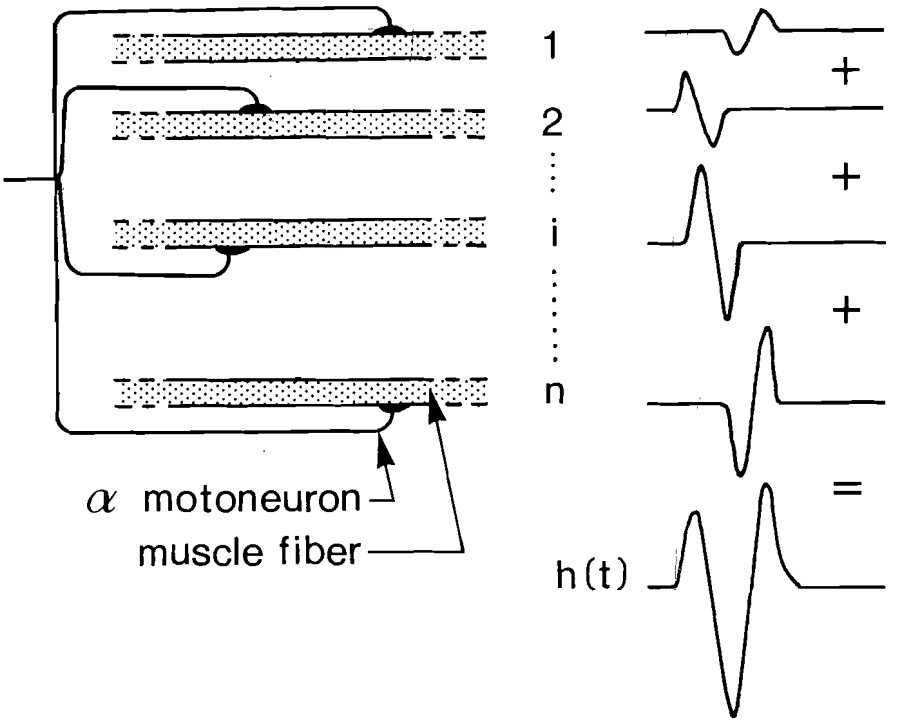
\includegraphics[width=0.6\linewidth]{./img/MUAP_oneMU.png}
\caption{Soma de potenciais de ação das \emph{n} fibras de uma unidade motora, formando uma MUAP \emph{h(t)}. Adaptado de BASMAJIAN e DE LUCA, 1985}
\label{fig:MUAP_comp}
\end{figure}
	
	Dependendo do método utilizado para aquisição de EMG, é comum a captura da contribuição de mais de uma unidade motora no mesmo canal. A influência de uma unidade motora no sinal adquirido depende principalmente da distância das fibras musculares ao ponto de aquisição (HAMMARBERG and STERNAD, 2002). A Figura \ref{fig:MUAP_soma} apresenta um exemplo com três unidades motoras, cujas MUAPs somadas compõem o sinal adquirido.
	
\begin{figure}
\centering
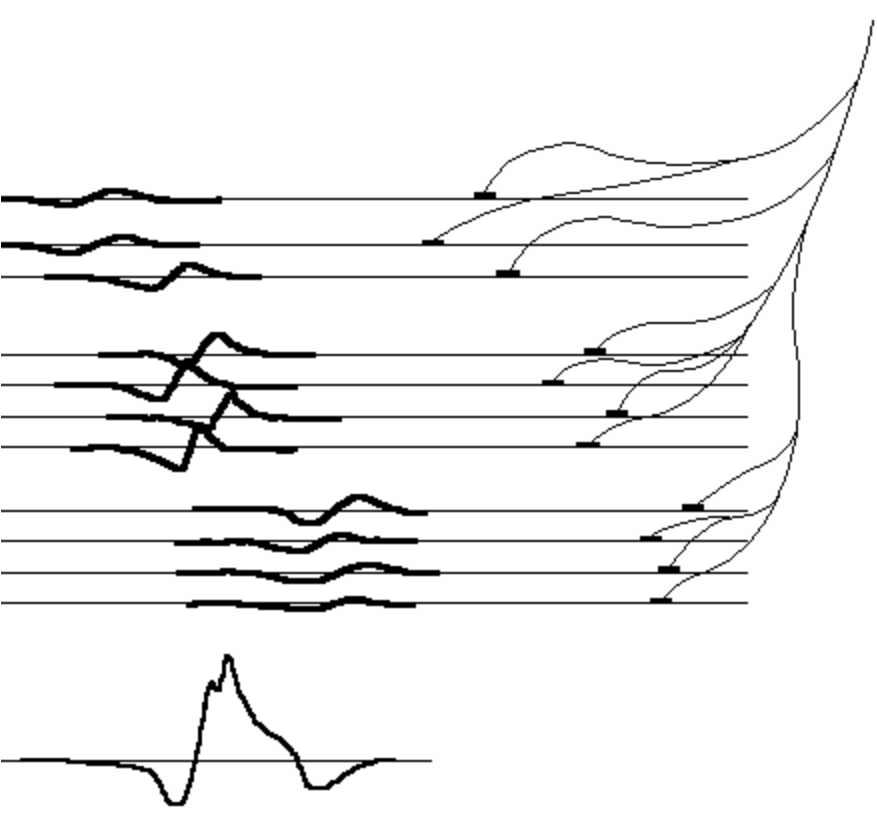
\includegraphics[width=0.6\linewidth]{./img/MUAP_soma.PNG}
\caption{Os sinais de MUAP correspondentes a três diferentes unidades motoras somam-se para formar o sinal adquirido por um canal de EMG. Adaptado de HAMMARBERG and STERNAD, 2002}
\label{fig:MUAP_soma}
\end{figure}
	
	Sinais de EMG de longa duração são constituídos por sequências temporais de MUAPs, também conhecidas como MUAPTs (\emph{MUAP Trains}). A Figura \ref{fig:MUAP_trains} exemplifica MUAPTs de diferentes MUs que somam-se para formar um sinal de EMG de longa duração.
	
\begin{figure}
\centering
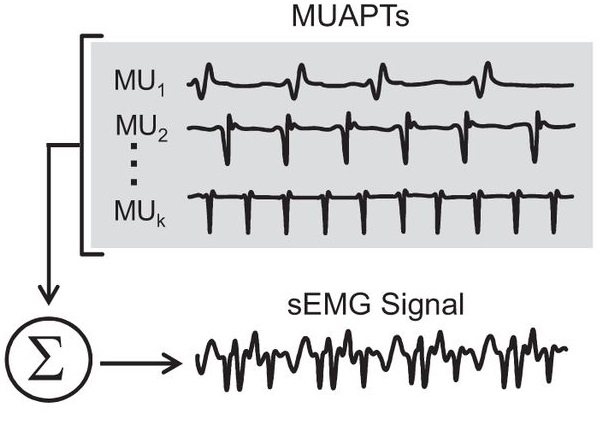
\includegraphics[width=0.6\linewidth]{./img/MUAP_trains.jpg}
\caption{MUAPTs de diferentes MUs somam-se para compor o sinal adquirido por um canal de EMG. Adaptado de KLINE and DE LUCA, 2014}
\label{fig:MUAP_trains}
\end{figure}

% ---
\section{Métodos de Segmentação}
% ---

	Esta seção descreve os métodos de segmentação originais que foram utilizados para basear os métodos implementados neste estudo. Nota-se que nomes utilizados para variáveis e constantes (e.g. `$r$', `$T$', etc.) foram determinados pelo autor deste estudo, não necessariamente sendo estes utilizados nos métodos originais. Para as definições dos métodos 3 e 4 (MTD3 e MTD4) são utilizados os termos BEP (\emph{beginning extraction point}, ponto inicial de um segmento) e EEP (\emph{ending extraction point}, ponto final de um segmento), também utilizados em (PATTICHIS et al, 1995).
	
% ---
\subsection{Método 1 (MTD1) - método iterativo para detecção de centros de segmentos de comprimento constante}
% ---

	Este é o método iterativo de segmentação utilizado em (CHAUVET et al, 2001). As definições da Tabela \ref{tab:mtd1params} serão utilizados para descrever este método.
	
\begin{table}[htb]
\IBGEtab{%
	\caption{Parâmetros utilizados para definir MTD1}%
	\label{tab:mtd1params}
}{%
	\begin{tabular}{ccc}
	\toprule
	Nome & Descrição \\
	\midrule \midrule
	$x$ & Sinal a ser segmentado \\
	\midrule
	$L$ & Comprimento total do sinal a ser segmentado \\
	\midrule
	$l$ & Comprimento desejado para os segmentos \\
	\midrule
	$T_k$ & Valor de \emph{threshold} para a iteração $k$ \\
	\midrule 
	$q$ & Fração de $T_{k-1}$ para determinação de $T_k$ \\
	\midrule 
	$N_{k}$ & Número total de candidatos para centros de segmentos identificados na iteração $k$ \\
	\midrule 
	$r_k$ & Razão entre número de candidatos identificados na iteração $k$ e o comprimento total do sinal \\
	\midrule 
	$r_{target}$ & Razão mínima esperada para $r_k$, utilizada para determinar o final do método \\
	\bottomrule
\end{tabular}%
}{%
	\fonte{Do autor.}%
}
\end{table}
	
	Inicialmente, determina-se o valor de \emph{threshold} $T_0$ equivalente ao máximo absoluto do sinal a ser segmentado $x$ (equação (\ref{eq:mtd1t0})). O valor $T_k$ é atualizado em cada iteração $k$ como sendo uma fração $q$ de $T_{k-1}$ (equação (\ref{eq:mtd1tk})). No trabalho de (CHAUVET et al, 2001), este valor $q$ é de 90\%.
	
\begin{equation}
\label{eq:mtd1t0}
  T_0 = max(x)
\end{equation}

\begin{equation}
\label{eq:mtd1tk}
  T_k = q \times T_{k-1}
\end{equation}

	Pontos do sinal acima do valor de $T_k$ são possíveis candidatos para centros de segmentos. Caso exista mais de um possível candidato em uma vizinhança bilateral de $l$ amostras do sinal, apenas o ponto de maior amplitude nesta vizinhança é considerado.
	
	Para determinar o final do método, avalia-se a razão $r_k$ entre a quantidade identificada de candidatos $N_{k}$ e o comprimento total do sinal $L$ (equação \ref{eq:mtd1rk}). Caso $r_k$ seja menor que um valor predeterminado $r_{target}$, calcula-se $T_{k+1}$ para realização da próxima iteração (equação \ref{eq:mtd1tk}). Caso $r_k$ seja maior ou igual ao valor predeterminado $r_{target}$, encerra-se o método e os segmentos são tomados como janelas de sinal de comprimento $l$, centradas nos candidatos identificados na última iteração.
	
\begin{equation}
\label{eq:mtd1rk}
  r_k = \frac{N_{k}}{L} 
\end{equation}
	
	O seguinte fluxograma resume os passos realizados para segmentação pelo MTD1.
	
\begin{tikzpicture}[node distance = 2cm, auto]
    % Place nodes
    \node [block] (init) {INÍCIO\\$k = 0$\\$T_0 = max(x)$};
    \node [block, below of=init, node distance=3cm] (identify) {Identificar candidatos a centros de segmentos};
    \node [decision, below of=identify] (decide) {$\frac{N_c}{L} >= r_{target}$};
	\node [block, left of=identify, node distance=6cm] (update) {$k++$\\$T_k = q \times T_{k-1}$};
    \node [block, below of=decide, node distance=4cm] (stop) {Segmentos de comprimento $l$ centrados nos candidatos identificados \\ FIM};
    % Draw edges
    \path [line] (init) -- (identify);
    \path [line] (identify) -- (decide);
    \path [line] (decide) -| node [near start] {NÃO} (update);
    \path [line] (update) |- (identify);
    \path [line] (decide) -- node {SIM}(stop);
	
	\label{fig:mtd1flux}
\end{tikzpicture}
	
	Para ilustrar o MTD1, a Figura \ref{fig:mtd1example} apresenta uma implementação em trecho de sinal de EMG retirado da base de dados Ninapro, com fração $q$ de 90\% (isto é, $T_k = 0.9\times T_{k-1}$) e segmentos de comprimento $l$ de 401 amostras.
 
\begin{figure}
\centering
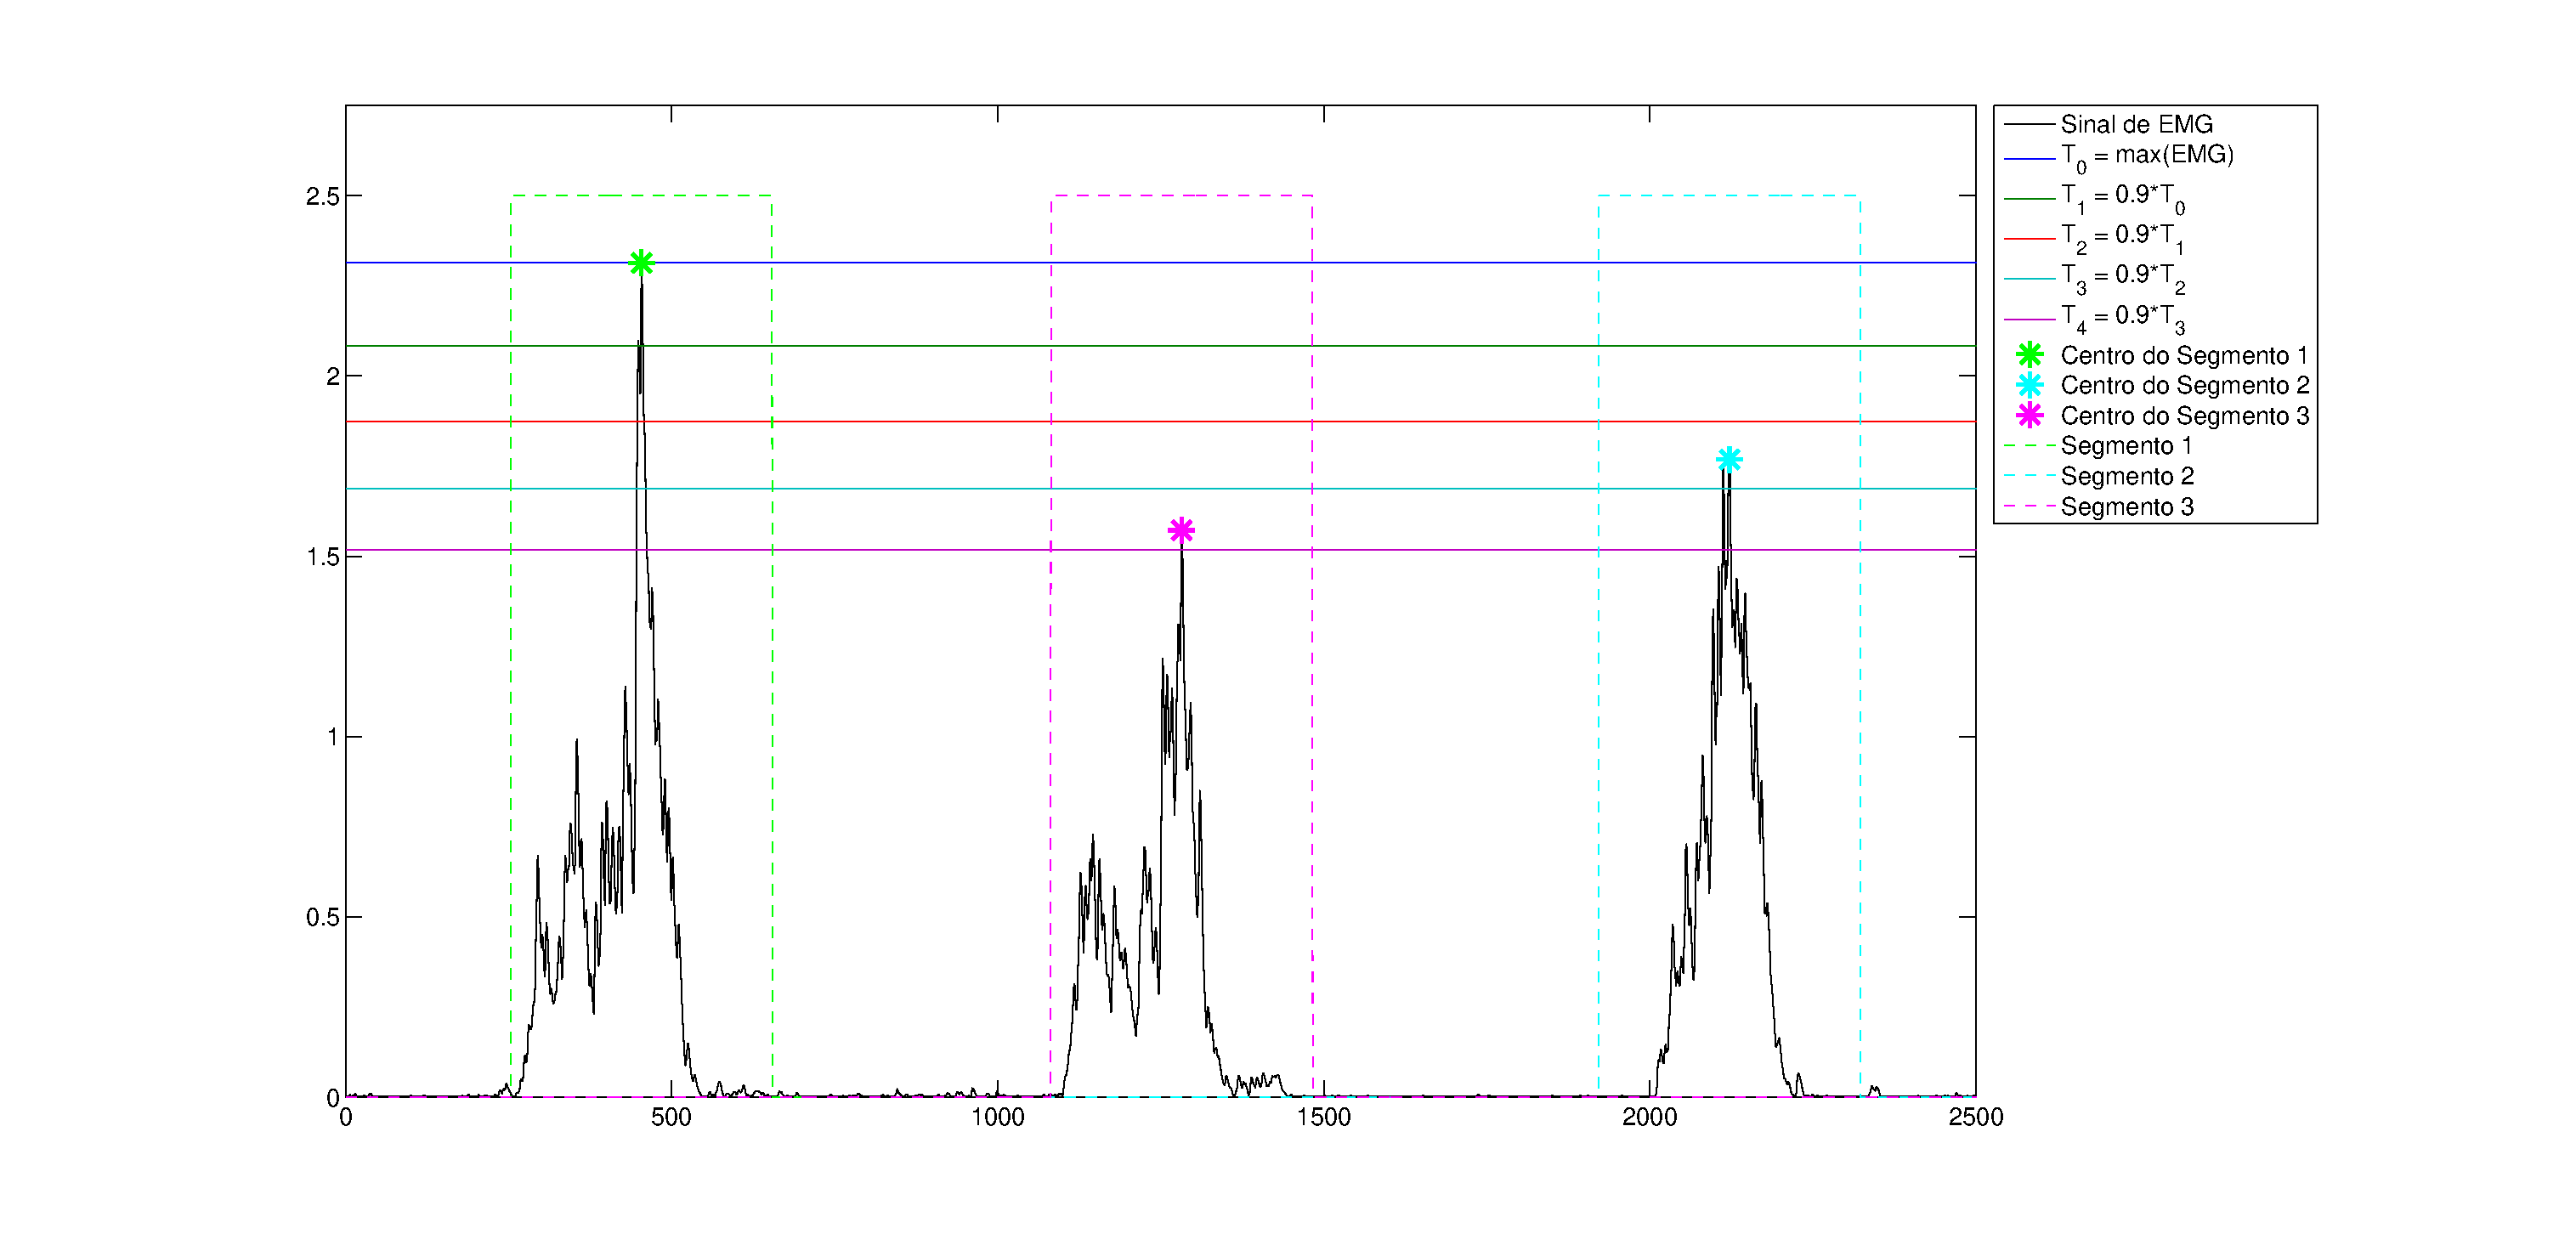
\includegraphics[width=\linewidth]{./img/mtd1example.eps}
\caption{Ilustração da implementação do MTD1, com $q = 0.9$ e $l = 401$. Do autor.}
\label{fig:mtd1example}
\end{figure}
 
% ---
\subsection{Método 2 (MTD2) - método não iterativo para detecção de centros de segmentos de comprimento constante}
% ---
	Este é o método de segmentação utilizado em (KATSIS et al, 2006). As definições da Tabela \ref{tab:mtd2params} serão utilizados para descrever este método. 
	
\begin{table}[htb]
\IBGEtab{%
	\caption{Parâmetros utilizados para definir MTD2}%
	\label{tab:mtd2params}
}{%
	\begin{tabular}{ccc}
	\toprule
	Nome & Descrição \\
	\midrule \midrule
	$x$ & Sinal a ser segmentado \\
	\midrule
	$L$ & Comprimento total do sinal a ser segmentado \\
	\midrule
	$l$ & Comprimento desejado para os segmentos \\
	\midrule
	$T$ & Valor de \emph{threshold} \\
	\bottomrule
\end{tabular}%
}{%
	\fonte{Do autor.}%
}
\end{table}
	
	Primeiramente, calcula-se o valor de \emph{threshold} $T$ a partir da média, do comprimento $L$ e do valor máximo do sinal a ser segmentado $x$. No trabalho de (KATSIS et al, 2006), a relação utilizada para cálculo de $T$ é dada em (\ref{eq:thKatsisCond}).

\begin{equation}
\label{eq:thKatsisCond}
	if\left(max(x) > \frac{30}{L}\sum_{i=1}^{L}|x_i|\right); then: T = \frac{5}{L}\sum_{i=1}^{L}|x_i|; else: T = \frac{max(x)}{5}
\end{equation}

	De forma similar ao MTD1, os pontos do sinal que tiverem valor acima de $T$ são considerados possíveis candidatos para centros de segmentos. Para os possíveis candidatos que estiverem afastados de uma distância inferior a $l$, apenas o candidato de maior amplitude é considerado. Em (KATSIS et al, 2006) utilizou-se comprimento $l$ de 121 amostras.
	
	A Figura \ref{fig:mtd1example} serve para ilustrar o MTD2, apresentando uma implementação em trecho de sinal de EMG retirado da base de dados Ninapro, com segmentos de comprimento $l$ de 401 amostras. O valor de \emph{threshold} T para este exemplo é calculado como $T = \frac{max(x_i)}{5}$, já que o máximo absoluto do sinal é menor que trinta vezes a média do sinal.

\begin{figure}
\centering
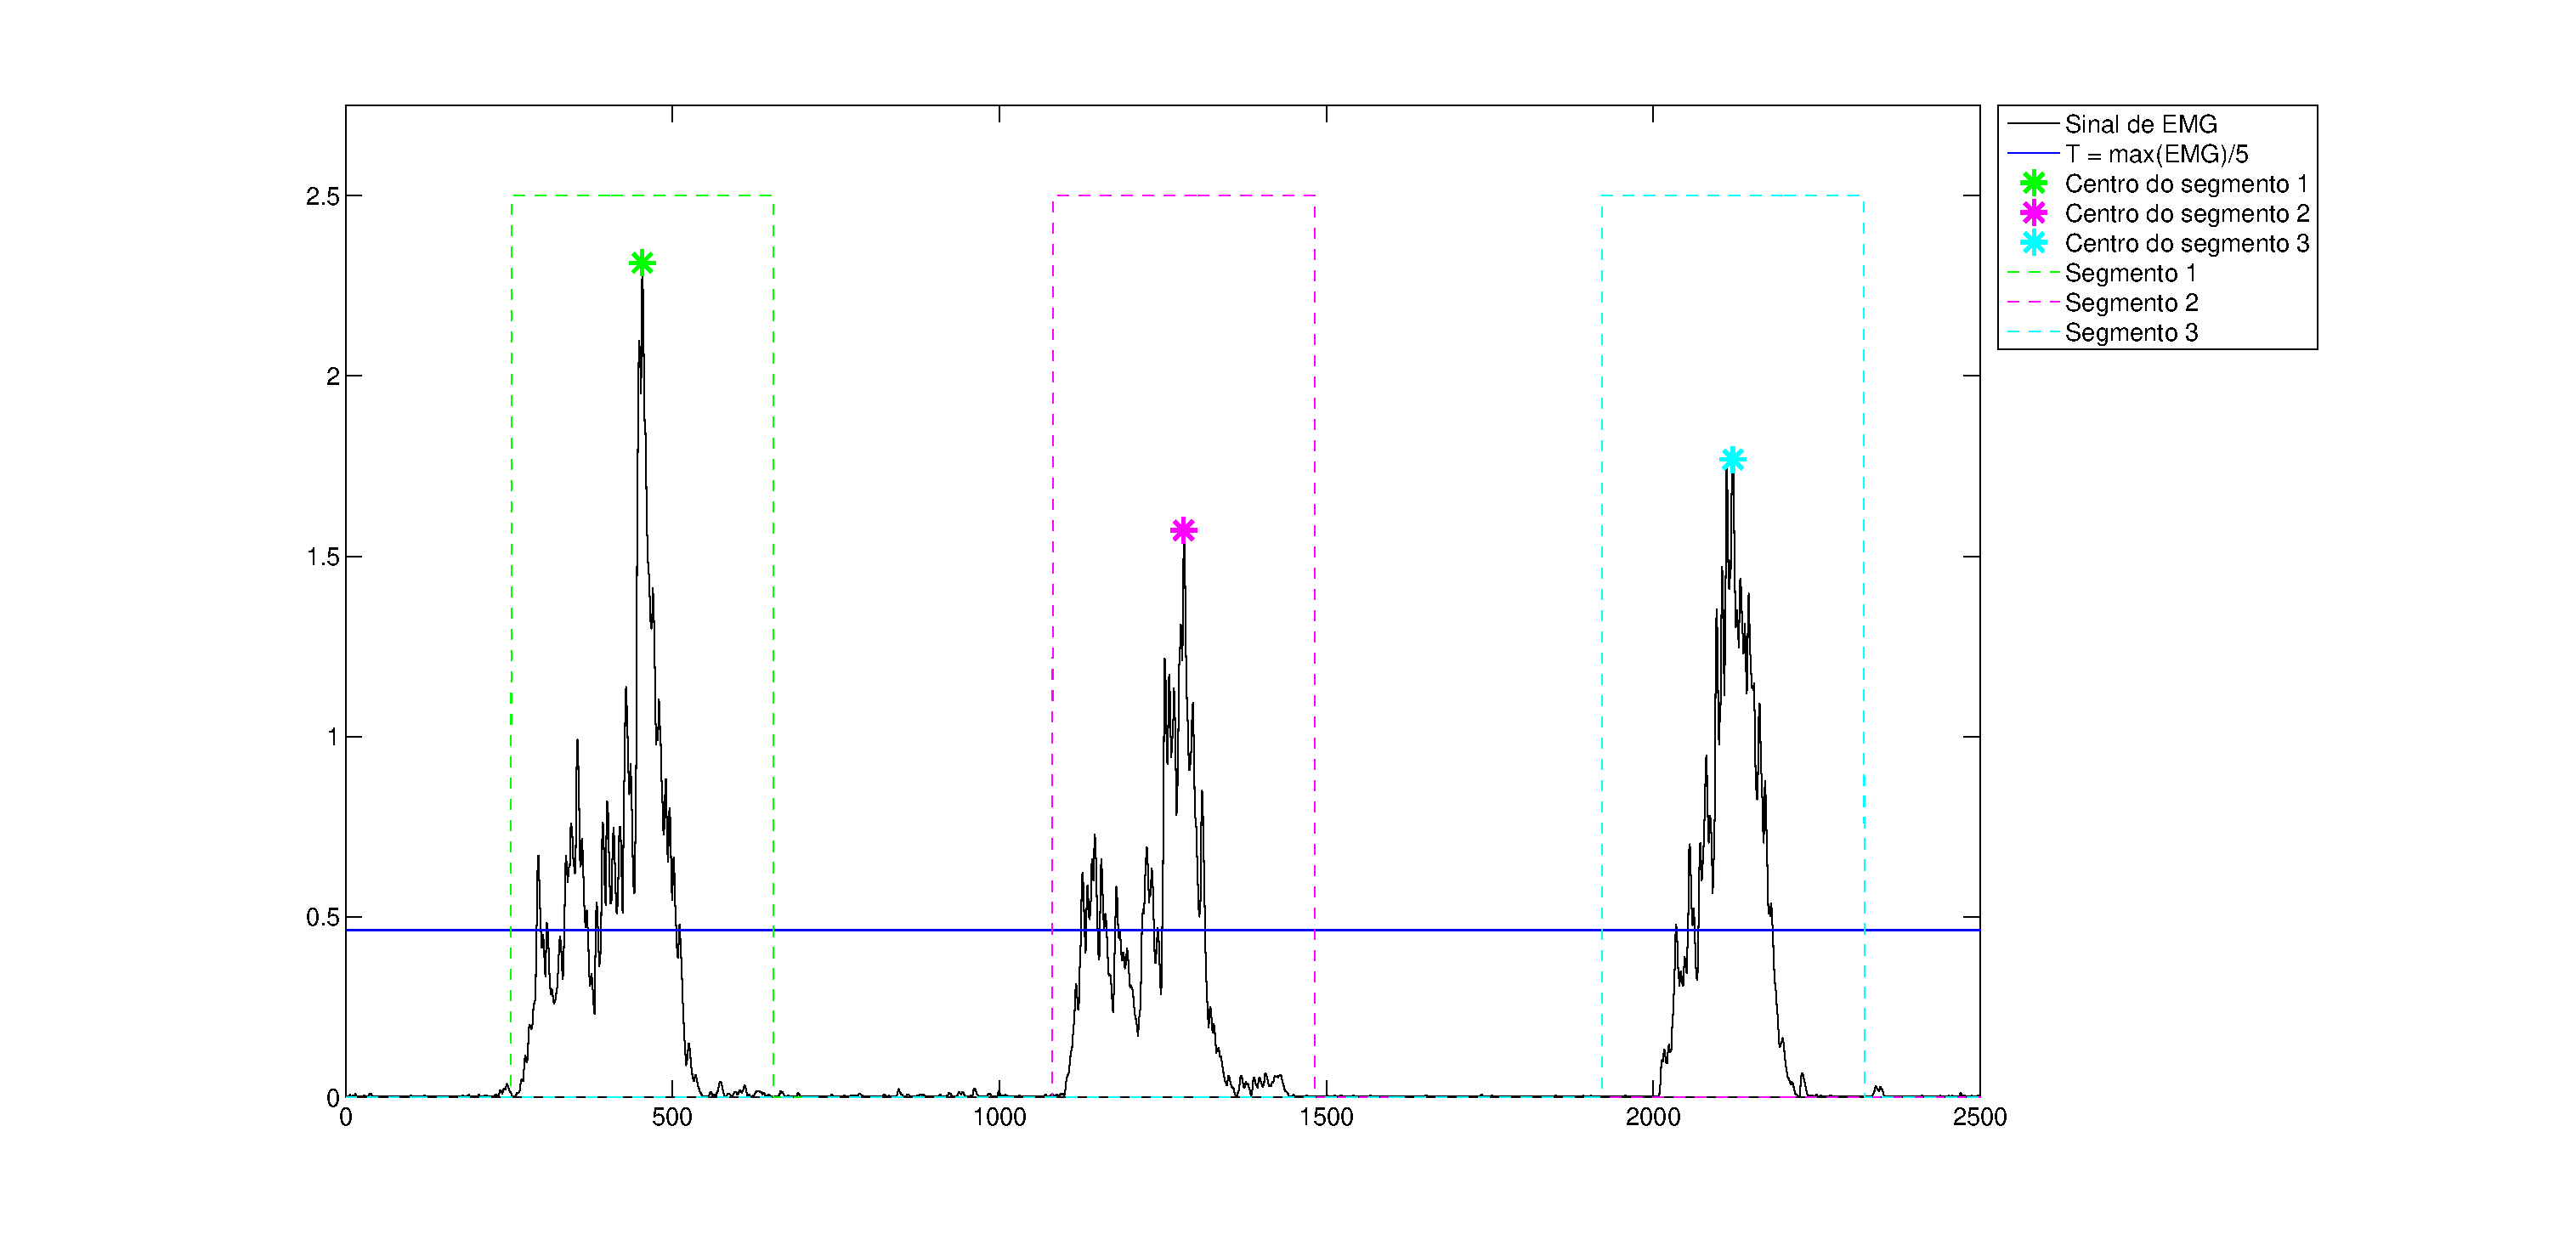
\includegraphics[width=\linewidth]{./img/mtd2example.eps}
\caption{Ilustração da implementação do MTD2, com $l = 401$. Do autor.}
\label{fig:mtd2example}
\end{figure}
	
% ---
\subsection{Método 3 (MTD3) - método com janela deslizante para detecção de BEP e EEP de segmentos utilizando variação total}
% ---

	Este é o método de segmentação utilizado em (GUT and MOSCHYTZ, 2000). As definições da Tabela \ref{tab:mtd3params} serão utilizados para descrever este método.
	
\begin{table}[htb]
\IBGEtab{%
	\caption{Parâmetros utilizados para definir MTD3}%
	\label{tab:mtd3params}
}{%
	\begin{tabular}{ccc}
	\toprule
	Nome & Descrição \\
	\midrule \midrule
	$x$ & Sinal a ser segmentado \\
	\midrule
	$W$ & Comprimento da janela deslizante utilizada pelo método \\
	\midrule
	$w_0$ & Número da amostra mais a esquerda da janela. Determina a posição instantânea da janela \\
	\midrule
	$\beta$ & Declividade média do sinal $x$ contido na janela deslizante \\
	\midrule
	$B$ & Valor limite para declividade média que determina ponto inicial de um segmento\\
	\midrule
	$\gamma$ & Variação total do sinal $x$ contido na janela deslizante \\
	\midrule
	$C$ & Valor limite para variação total que determina ponto final de um segmento\\
	\bottomrule
\end{tabular}%
}{%
	\fonte{Do autor.}%
}
\end{table}
	
	Uma janela deslizante de comprimento $W$ percorre o sinal da esquerda para a direita. Caso a declividade média $\beta$ do trecho de sinal contido pela janela, calculado pela equação (\ref{eq:decMedia}), exceda um limite $B$, o ponto mais à esquerda da janela $w_0$ determina a BEP de um segmento.
	
\begin{equation}
\label{eq:decMedia}
	\beta = \frac{1}{W}\sum_{i=w_0+1}^{W}(x_i - x_{i-1})
\end{equation}
	
	O EEP do correspondente segmento é então obtido como o ponto mais à direita da janela ($w_0 + W - 1$) quando a variação total $\gamma$, dado pela equação (\ref{eq:varTotal}), do trecho de sinal contido pela janela for menor que um limite $C$.

\begin{equation}
\label{eq:varTotal}
	\gamma = \sum_{i=w_0+1}^{W}(x_i - x_{i-1})
\end{equation}
	
	Nota-se que as equações (\ref{eq:decMedia}) e (\ref{eq:varTotal}) diferem somente pela divisão pelo comprimento da janela $W$ em (\ref{eq:decMedia}). Com valores adequados para os limites $B$ e $C$, o MTD3 pode ser implementado utilizando apenas uma destas equações. A Figura \ref{fig:mtd3example} exemplifica uma janela deslizante que determina BEPs e EEPs de segmentos utilizando o MTD3.
	
\begin{figure}
\centering
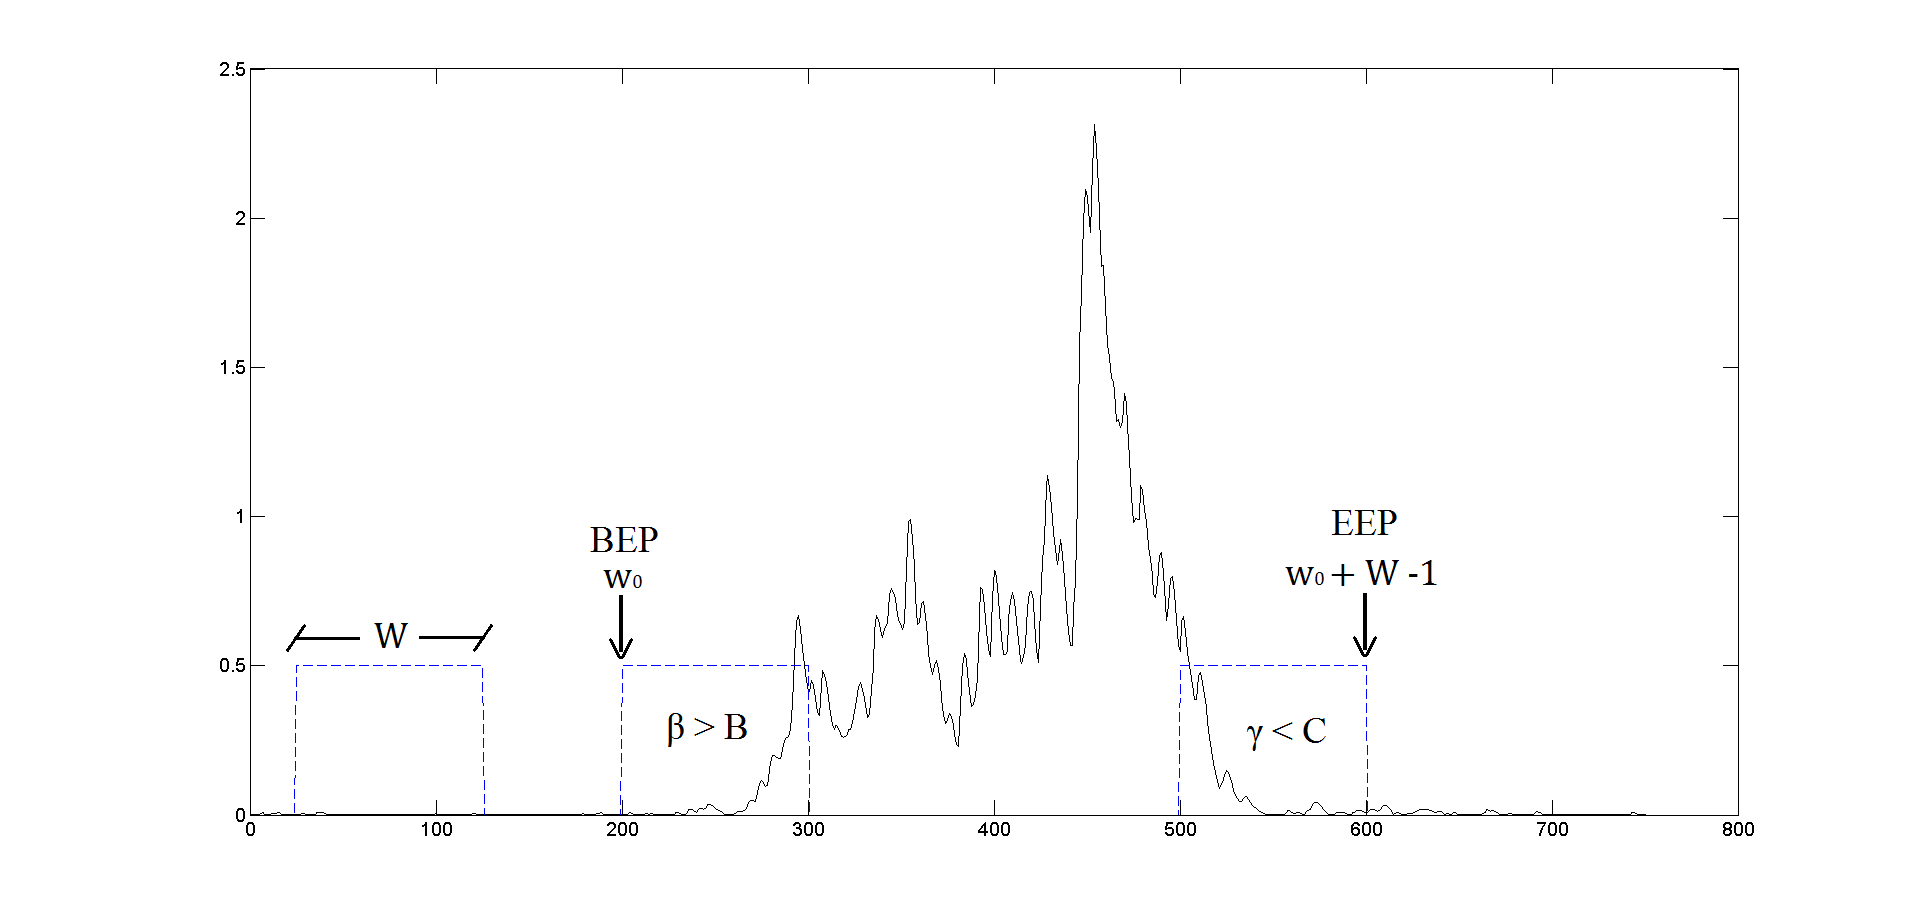
\includegraphics[width=\linewidth]{./img/mtd3ex.png}
\caption{Ilustração da implementação do MTD3, com $W = 100$. Do autor.}
\label{fig:mtd3example}
\end{figure}
	
% ---
\subsection{Método 4 (MTD4) - método com janela deslizante para detecção de BEP e EEP de segmentos utilizando \emph{threshold}}
% ---

Este é o método de segmentação utilizado em (PACHITTIS et al, 1995). As definições da Tabela \ref{tab:mtd4params} serão utilizados para descrever este método.
	
\begin{table}[htb]
\IBGEtab{%
	\caption{Parâmetros utilizados para definir MTD4}%
	\label{tab:mtd4params}
}{%
	\begin{tabular}{ccc}
	\toprule
	Nome & Descrição \\
	\midrule \midrule
	$x$ & Sinal a ser segmentado \\
	\midrule
	$W$ & Comprimento da janela deslizante utilizada pelo método \\
	\midrule
	$T$ & Valor de \emph{threshold} \\
	\bottomrule
\end{tabular}%
}{%
	\fonte{Do autor.}%
}
\end{table}
	
	Primeiramente, a janela deslizante de comprimento $W$ percorre o sinal da direita para a esquerda. Os BEPs dos segmentos são os primeiros pontos (com exceção do final do sinal $x$) nas quais, com a janela situada à esquerda do ponto, o sinal contido pela janela permanece abaixo do valor de threshold $T$.
	
	As EEPs são identificadas de forma similar, com a janela percorrendo o sinal da esquerda para a direita. Os EEPs dos segmentos são os primeiros pontos nas quais, com a janela situada à direita do ponto (com exceção do ínicio do sinal $x$), o sinal contido pela janela permanece abaixo do valor de threshold $T$.
	
	No trabalho de (PACHITTIS et al, 1995), utilizou-se janelas de comprimento $W$ correspondente a 3 $ms$ de aquisição e \emph{threshold} $T$ de $\pm$ 40 $\mu V$ (o sinal de EMG segmentado não era retificado). A Figura \ref{fig:mtd4example} exemplifica as determinações de BEPs e EEPs utilizando o MTD4.
	
\begin{figure}
\centering
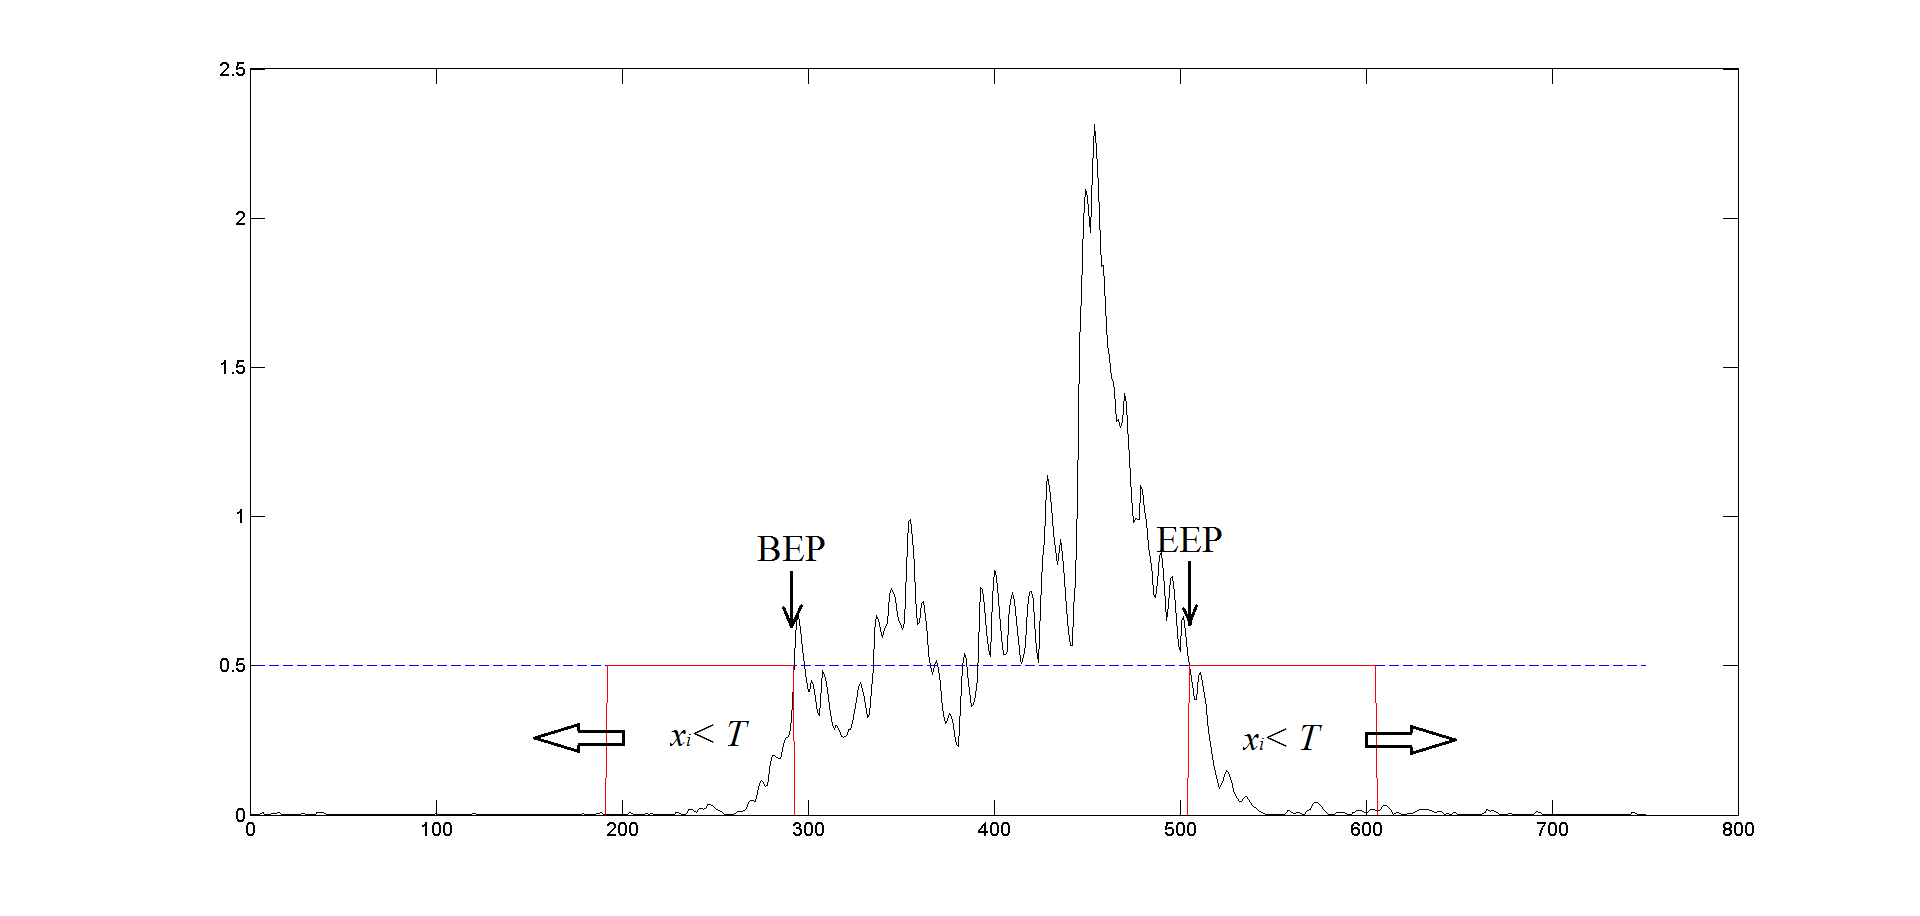
\includegraphics[width=\linewidth]{./img/mtd4ex.png}
\caption{Ilustração da implementação do MTD4, com $W = 100$ e $T = 0,5$. Do autor.}
\label{fig:mtd4example}
\end{figure}

% ---
\section{Redes Neurais Artificias}
% ---

	TODO: REVISÃO SOBRE REDES NEURAIS
